% Source: Lecture4.pdf, pages 1-9.
\lecture{4}
\subsubsection*{Three-dimensional crystal structures}

Recall some 3D crystal structures (the cubic cells are drawn in
Figure~\ref{fig:cubic}):
\begin{center}
\begin{tabular}{lll}
  structure & coord.\ no. & \\ \hline
  simple cubic, sc & 6 & \\
  body-centered cubic, bcc & 8 & with a site in the middle of the cube\\
  face-centered cubic, fcc & 12 & with sites at the centers of the faces\\
  hexagonal close packed, hcp & 12 &
\end{tabular}
\end{center}
E.g.\ the solid phase of Ar, Ne at $p\sim 1$~atm is fcc.

\subsubsection*{Two-dimensional lattices}

The homopolygonal 2D lattices are the square lattice (sq), coordination number 4,
$(4^4)$; the triangular lattice (tri), coordination number 6, $(3^6)$; and the
honeycomb (hc) or hexagonal lattice, coordination number 3, $(6^3)$. Some
heteropolygonal Archimedean lattices (2D) are the $(4\cdot 8\cdot 8)$ lattice,
coordination number 3, and the $(3\cdot 6\cdot 3\cdot 6)$ kagom\'e lattice,
coordination number 4.

\begin{diagram}
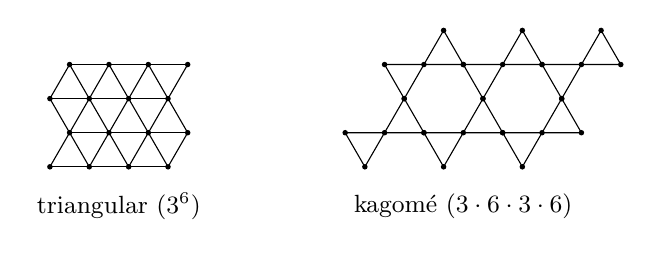
\begin{tikzpicture}[scale=0.5]
  % triangular
  \foreach \j in {0,1,2,3} \foreach \i in {0,1,2,3} {
    \pgfmathsetmacro{\x}{\i + 0.5*mod(\j,2)}
    \pgfmathsetmacro{\y}{0.866*\j}
    \fill (\x,\y) circle (0.07);
  }
  \foreach \j in {0,1,2,3} \draw ({0.5*mod(\j,2)},{0.866*\j}) -- ++(3,0);
  \foreach \i in {0,1,2,3} {\draw (\i,0) -- ++(60:1) -- ++(120:1) -- ++(60:1);}
  \foreach \i in {1,2,3} {\draw (\i,0) -- ++(120:1) -- ++(60:1) -- ++(120:1);}
  \node[font=\small] at (1.75,-1) {triangular $(3^6)$};
  % kagome: the medial graph of a triangular lattice of edge 2; corner-sharing triangles around hexagons
  \begin{scope}[xshift=7cm]
    \foreach \j in {0,1} \foreach \i in {0,1,2} {
      \begin{scope}[shift={(2*\i+\j,1.732*\j)}]
        \draw (1,0) -- (1.5,0.866) -- (0.5,0.866) -- cycle;
        \draw (1.5,0.866) -- (2.5,0.866) -- (2,1.732) -- cycle;
        \foreach \p in {(1,0),(0.5,0.866),(1.5,0.866),(2.5,0.866),(2,1.732)} \fill \p circle (0.07);
      \end{scope}}
    \node[font=\small] at (3.5,-1) {kagom\'e $(3\cdot 6\cdot 3\cdot 6)$};
  \end{scope}
\end{tikzpicture}
\diagramcaption{The triangular lattice and the kagom\'e lattice. The square,
honeycomb and $4\cdot 8^2$ lattices are drawn in Figures~\ref{fig:duality}
and~\ref{fig:488}.}
\end{diagram}

\subsection{Helium-4 and universality classes}
\subsubsection*{Helium-4}

Another phase diagram: $^4$He, the lightest noble element. This has the property that
there is no solid phase at pressure $p\sim 1$~atm; one has to increase $p\gtrsim 25$~atm
to get the $^4$He to solidify. This is due to large quantum zero-point motions of the He
atoms. Another important property is a phase transition (of second order) between a
normal liquid and a superfluid that flows without viscosity: a manifestation of
Bose--Einstein condensation.

\begin{diagram}
\begin{tikzpicture}[scale=1.0,>=Stealth]
  \draw (0,0) -- (8,0) node[below right] {$T$};
  \draw (0,0) -- (0,4.6) node[left] {$p$};
  % solid boundary at ~25 atm, lambda line, liquid-gas curve
  \draw[thick] (0,3.0) -- (2.0,3.0) .. controls (3.2,3.25) and (4.8,3.8) .. (6.0,4.5);
  \draw[thick] (2.0,3.0) .. controls (2.1,2.3) and (2.2,1.6) .. (2.25,1.0);
  \draw[thick] (1.0,0.15) .. controls (1.6,0.55) and (1.95,0.8) .. (2.25,1.0);
  \draw[thick] (2.25,1.0) .. controls (3.4,1.35) and (5.0,1.8) .. (6.6,2.2);
  \fill (6.6,2.2) circle (0.06);
  \draw[dotted] (0,1.3) -- (3.3,1.3);
  \draw[dotted] (2.25,1.0) -- (2.25,0); \draw[dotted] (3.3,1.3) -- (3.3,0); \draw[dotted] (6.6,2.2) -- (6.6,0);
  \node[left,font=\small] at (0,3.0) {25 atm};
  \node[left,font=\small] at (0,1.3) {1 atm};
  \node[below,font=\small] at (2.2,0) {2.18};
  \node[below,font=\small] at (3.3,0) {4.22};
  \node[below,font=\small] at (6.6,0) {5.195 K};
  \node[font=\small] at (1.0,3.8) {solid hcp};
  \node[font=\small] at (2.9,3.7) {bcc};
  \node[font=\small] at (1.05,2.0) {superfluid};
  \node[font=\small] at (4.0,2.6) {normal liquid};
  \node[font=\small,anchor=west] at (2.3,2.2) {$\lambda$ line};
  \node at (6.0,0.7) {gas};
  \node[anchor=west,font=\small] at (6.7,2.45) {critical pt.};
  \node[anchor=west,font=\small] at (5.2,3.4) {$T_c = 5.195$ K, $p_c = 2.25$ atm};
  \node[anchor=west,font=\small] at (3.4,1.0) {$T_b = 4.22$ K};
  \node[font=\small] at (1.0,0.95) {$T_\lambda = 2.177$ K}; \draw[->] (1.85,0.95) -- (2.19,0.99);
\end{tikzpicture}
\diagramcaption{Phase diagram of $^4$He ($T_b = 4.222$~K). The $\lambda$ line separates
the superfluid from the normal liquid.}
\end{diagram}

The ``$\lambda$'' line is named for the shape of the specific heat curve (see, e.g.,
Stanley, p.~20, Fig.~1.16).

\begin{diagram}
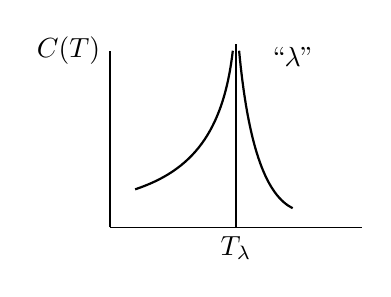
\begin{tikzpicture}[scale=0.8]
  \draw (0,0) -- (4,0); \draw (0,0) -- (0,2.8) node[left] {$C(T)$};
  \draw (2,0) -- (2,2.9);
  \draw[thick] (0.4,0.6) .. controls (1.3,0.9) and (1.8,1.5) .. (1.95,2.8);
  \draw[thick] (2.05,2.8) .. controls (2.2,1.2) and (2.5,0.5) .. (2.9,0.3);
  \node[below] at (2,0) {$T_\lambda$};
  \node at (2.9,2.7) {``$\lambda$''};
\end{tikzpicture}
\diagramcaption{The specific heat of $^4$He near $T_\lambda$.}
\end{diagram}

The physical origin of ferromagnetism is due to the Pauli Exclusion Principle: if spins
are aligned, then the electron clouds do not overlap, and the resultant separation
reduces the Coulomb energy due to e--e electrostatic repulsion. Antiferromagnetism occurs
due to a combination of this effect and spin interactions in compounds, e.g.\ MnO, etc.

\subsubsection*{Universality classes of phase transitions}

\paragraph{1. Uniaxial ferromagnet (Ising model), \texorpdfstring{$G = \mathbb{Z}_2$}{G = Z2}.}

\begin{equation}
  \Ham = -J\sum_{\langle ij\rangle}\sigma_i\sigma_j - \mu H\sum_i\sigma_i ,
\end{equation}
where $\sigma_i = \pm 1$ is a classical spin and $J$ is the spin--spin exchange
(coupling). Here $\mathbf{S}_i = (1/2)\boldsymbol{\sigma}_i$, and we absorb
$(1/2)^2$ into $J$. The second term comes from
$U_{\text{mag}} = -\boldsymbol{\mu}\cdot\mathbf{H}$; choose units such that $\mu = 1$.
\begin{itemize}
  \item $J>0\Rightarrow$ the spin--spin interaction favors parallel spins,
    $\uparrow\uparrow$: FM (ferromagnetic sign of the coupling).
  \item $J<0$ favors opposite orientations of nearest-neighbor (n.n.) spins,
    $\uparrow\downarrow$: AFM.
\end{itemize}
The symmetry (group) of this $\Ham$ with $H = 0$ (i.e.\ zero external magnetic field) is
$\mathbb{Z}_2$, generated by $\{1,-1\}$ (the identity, and $\uparrow\to\downarrow$). A
$\mathbb{Z}_2$ transformation reverses all spins (a global symmetry operation):
\begin{equation}
  \sigma_i\sigma_j\to(-\sigma_i)(-\sigma_j) = \sigma_i\sigma_j .
\end{equation}
This symmetry is explicitly broken if the external field $H\ne 0$. As $T\searrow T_c$
(given that $H = 0$) the $\mathbb{Z}_2$ symmetry is spontaneously broken by the onset of
a spontaneous magnetization.

\begin{diagram}
\begin{tikzpicture}[scale=0.8]
  \draw (0,0) -- (4,0); \draw (0,0) -- (0,2.4) node[left] {$M_{sp}(T)$};
  \draw[thick] (0,1.9) -- (0.9,1.9) .. controls (2.2,1.85) and (2.9,1.3) .. (3,0);
  \node[below] at (1,0) {$T$}; \node[below] at (3,0) {$T_c$};
\end{tikzpicture}
\diagramcaption{Onset of spontaneous magnetization below $T_c$.}
\end{diagram}

SSB = spontaneous symmetry breaking, associated with LRO = long-range order and a nonzero
value of the order parameter, which is the spontaneous magnetization.

\paragraph{2. Liquid--gas: an example of the \texorpdfstring{$\mathbb{Z}_2$}{Z2} universality class.}

The liquid--gas (also liquid--solid) phase transition. Imagine a formal lattice (the
lattice gas model of T.D.~Lee and C.N.~Yang). Say pressure $p$ is fixed. At $T>T_c$, the
probability of a molecule or atom being present at a site in the lattice gas is
$1/2$: random. As $T\searrow T_c$, the sites are occupied with probability $>1/2$.
As $T$ decreases further, this probability increases, $\to 1$.

\begin{diagram}
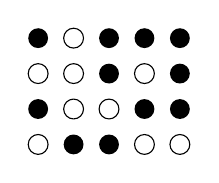
\begin{tikzpicture}[scale=0.45]
  \foreach \r/\row in {0/{1,0,1,1,1},1/{0,0,1,0,1},2/{1,0,0,1,1},3/{0,1,1,0,0}} {
    \foreach \v [count=\c] in \row {
      \ifnum\v=1 \fill (\c,-\r) circle (0.28); \else \draw (\c,-\r) circle (0.28); \fi
    }}
\end{tikzpicture}
\diagramcaption{A lattice gas: filled circles are occupied sites, open circles are
empty.}
\end{diagram}

The feature is yes/no with respect to occupation. It can be modelled as a phase
transition in the $\mathbb{Z}_2$ universality class. This model is justified a
posteriori by the agreement of the critical exponents calculated for a $\mathbb{Z}_2$
system and the experimentally measured values, e.g.\ recall the curve showing data at
$p_c$, $T_c$ for $\Delta\rho = \rho_\ell-\rho_g$ from Guggenheim.

\paragraph{3. \texorpdfstring{$O(N)$}{O(N)} spin models.}

For spin systems, we have (infinitely many) additional universality classes. Consider
the Hamiltonian
\begin{equation}
  \Ham = -J\sum_{\langle ij\rangle}\mathbf{S}_i\cdot\mathbf{S}_j
         - \mu\,\mathbf{H}\cdot\sum_i\mathbf{S}_i
\end{equation}
(again, choose units such that $\mu = 1$). Here $\mathbf{S}_i$ is a spin (a classical
vector with $|\mathbf{S}_i| = 1$, or quantum with $\|\mathbf{S}\|^2 = S(S+1)$, $\hbar = 1$)
with $N$ components, $\mathbf{S}_i = (S_{i,1},\ldots,S_{i,N})$.
\begin{itemize}
  \item $N = 3$ components: the Heisenberg model, $(S_{i,1},S_{i,2},S_{i,3})$. If
    $\mathbf{H} = 0$, the global symmetry group of $\Ham$ is $O(3)$.
  \item $O(2)$, $XY$, $N = 2$ components: $\mathbf{S}_i = (S_{i,1},S_{i,2})$. Here, as the
    name indicates, $G = O(2)$; the spin lives on $S^1$.
  \item In general, the $O(N)$ spin model. Recall that an $O(3)$ spin ``lives'' on $S^2$.
\end{itemize}
Definition: given a vector $\mathbf{x}\in\mathbb{R}^N$, the condition
$|\mathbf{x}| = \text{const.}$ defines the $(N-1)$-dimensional sphere $S^{N-1}$.

Similarly, for $O(N)$, $\mathbf{S}_i = (S_{i1},\ldots,S_{iN})$ with $|\mathbf{S}| = 1$
``lives'' on $S^{N-1}$, the $(N-1)$-sphere. A slice of the $S^2$ sphere is $\sim S^1$.
Similarly, a slice of $S^1$ is $\sim\mathbb{Z}_2$ (the two antipodal points in $S^1$). In
this sense, the Ising model is a member of the $O(N)$ series of models, corresponding to
$N = 1$.

An example of an $O(2)$ model: $O(2)\approx U(1)$, the group of elements $e^{\ii\theta}$
under multiplication, $e^{\ii\theta_1}\cdot e^{\ii\theta_2} = e^{\ii(\theta_1+\theta_2)}$.
In superconductivity the order parameter is the Cooper pair; in BCS theory
$\ev{ee}\sim\ev{\psi\psi}$, which has a complex phase. The superconducting phase
transition is in the $O(2)$ universality class. The normal fluid--superfluid phase
transition in $^4$He is also in the $O(2)\approx U(1)$ universality class; the order
parameter is the complex phase of the superfluid condensate wavefunction.

\paragraph{4. Structural transition in a binary alloy, \texorpdfstring{$\mathbb{Z}_2$}{Z2}.}

$\beta$ brass is an alloy of Cu and Zn (copper and zinc), on a body-centered cubic lattice.
At $T<T_c = 742$~K the Cu and Zn atoms are on the two interleaved sublattices. Recall
that the bcc lattice is bipartite, $\Lambda_{bcc} = \Lambda_e\oplus\Lambda_o$. As
$T\nearrow T_c$, the positions of the Cu and Zn atoms become increasingly random.

\begin{diagram}
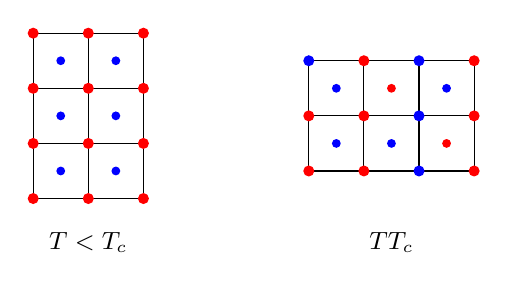
\begin{tikzpicture}[scale=0.7]
  \foreach \x in {0,1,2} \draw (\x,0) -- (\x,3);
  \foreach \y in {0,1,2,3} \draw (0,\y) -- (2,\y);
  \foreach \x in {0,1,2} \foreach \y in {0,1,2,3} \fill[red] (\x,\y) circle (0.1);
  \foreach \x in {0.5,1.5} \foreach \y in {0.5,1.5,2.5} \fill[blue] (\x,\y) circle (0.08);
  \node[font=\small,align=center] at (1,-0.8) {$T<T_c$};
  \begin{scope}[xshift=5cm,yshift=0.5cm]
    \foreach \x in {0,1,2,3} \draw (\x,0) -- (\x,2);
    \foreach \y in {0,1,2} \draw (0,\y) -- (3,\y);
    \foreach \x/\y/\c in {0/0/red,1/0/red,2/0/blue,3/0/red,0/1/red,1/1/red,2/1/blue,3/1/red,0/2/blue,1/2/red,2/2/blue,3/2/red}
      \fill[\c] (\x,\y) circle (0.1);
    \foreach \x/\y/\c in {0.5/0.5/blue,1.5/0.5/blue,2.5/0.5/red,0.5/1.5/blue,1.5/1.5/red,2.5/1.5/blue}
      \fill[\c] (\x,\y) circle (0.08);
    \node[font=\small] at (1.5,-1.3) {$T\gtrsim T_c$};
  \end{scope}
\end{tikzpicture}
\diagramcaption{Slices of the bcc lattice of $\beta$ brass, with Cu in red and Zn in
blue. Left: a portion of the bcc lattice at $T<T_c$. Right: a slice at $T\gtrsim T_c$,
showing the partial reduction in positional ordering.}
\end{diagram}

\paragraph{5. Liquid crystals.}

We will also consider other types of phase transitions. One example will involve
topological ordering: the liquid crystal isotropic--nematic transition.
\begin{itemize}
  \item Isotropic phase: no positional ordering and also no orientational ordering.
  \item Nematic phase: no positional ordering but $\exists$ orientational ordering.
\end{itemize}
The space of the order parameter for a liquid crystal is $S^2/\mathbb{Z}_2$, because the
ends of the rod-like molecules are equivalent, so we ``mod out'' $S^2$ by $\mathbb{Z}_2$.
(Contrast with a FM, where the spins carry arrows.)

\begin{diagram}
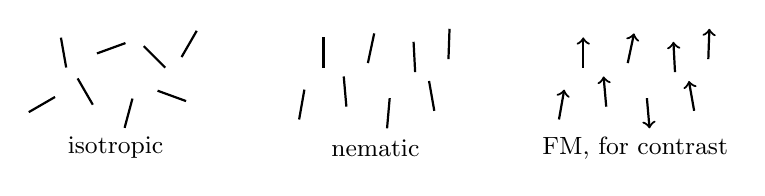
\begin{tikzpicture}[scale=0.55]
  \foreach \x/\y/\a in {0/0/30,1/0.3/120,2/-0.2/75,3/0.2/160,0.5/1.2/100,1.6/1.3/20,2.6/1.1/135,3.4/1.4/60}
    \draw[thick] (\x,\y) ++(\a:0.35) -- ++(\a+180:0.7);
  \node[font=\small] at (1.7,-1) {isotropic};
  \begin{scope}[xshift=6cm]
  \foreach \x/\y/\a in {0/0/80,1/0.3/95,2/-0.2/85,3/0.2/100,0.5/1.2/90,1.6/1.3/78,2.6/1.1/93,3.4/1.4/88}
    \draw[thick] (\x,\y) ++(\a:0.35) -- ++(\a+180:0.7);
  \node[font=\small] at (1.7,-1) {nematic};
  \end{scope}
  \begin{scope}[xshift=12cm]
  \foreach \x/\y/\a in {0/0/80,1/0.3/95,2/-0.2/-85,3/0.2/100,0.5/1.2/90,1.6/1.3/78,2.6/1.1/93,3.4/1.4/88}
    \draw[thick,->] (\x,\y) ++(\a+180:0.35) -- ++(\a:0.7);
  \node[font=\small] at (1.7,-1) {FM, for contrast};
  \end{scope}
\end{tikzpicture}
\diagramcaption{Rod-like molecules in the isotropic and nematic phases of a liquid
crystal, and spins in a ferromagnet.}
\end{diagram}

\subsubsection*{What determines the universality class}

So: the universality class of the critical point and associated second-order phase
transition is determined by
\begin{enumerate}[label=(\arabic*)]
  \item the symmetry group $G$ of the Hamiltonian $\Ham$;
  \item the spatial dimensionality of the lattice $\Lambda$.
\end{enumerate}
In the development of the theory of phase transitions and critical phenomena, this
notion of universality class was developed and tested by a combination of (a)
measurements on physical systems (recall the Guggenheim plot that showed the same
critical exponent $\beta$ for different gases, and similar measurements of different
magnetic systems); (b) approximate studies of model systems such as high-temperature
and low-temperature series expansions; (c) renormalization group analyses; (d) Monte
Carlo simulations.

Thus, for example, if we changed the Hamiltonian of the Ising model from
\begin{equation}
  \Ham = -J\sum_{\langle ij\rangle}\sigma_i\sigma_j - H\sum_i\sigma_i
\end{equation}
with, say, $J>0$ (FM), where $\langle ij\rangle$ are nearest-neighbor pairs of sites, to
include FM next-nearest-neighbor spin--spin interactions,
\begin{equation}
  \Ham_{nn+nnn} = -J_{nn}\sum_{\langle ij\rangle_{nn}}\sigma_i\sigma_j
                  - J_{nnn}\sum_{\langle k\ell\rangle_{nnn}}\sigma_k\sigma_\ell
                  - H\sum_i\sigma_i ,
\end{equation}
then the critical behavior is the same (again with $H = H_c = 0$), because the
$\mathbb{Z}_2$ (global) symmetry group of the zero-field $\Ham$ is the same and the
dimensionality of the lattice is, of course, unchanged. The $\Ham$ with nearest-neighbor
spin--spin interactions is a simplification, but usually a reasonably good one, since
interactions decrease as the distance between the spins (really the electron clouds)
increases.

Another condition to remain in the same universality class is that the additional
interactions are not ``competing interactions'' that introduce frustration. For example
if $J_{nn}>0$ (FM) but the nnn interaction had $J_{nnn}<0$ (AFM), this would be a
competing interaction: the $J_{nn}$ would favor spin alignment, but the $J_{nnn}$ would
favor antiparallel spin ordering, a conflicting tendency. This would lead to frustration
and would change the universality class.

One can also add multispin interactions such as 4-spin interactions involving the 4
spins on the sites of a square lattice (with $J_\square>0$ to avoid competing
interactions), to get
\begin{equation}
  \Ham = -J_{nn}\sum_{\langle ij\rangle}\sigma_i\sigma_j
         - J_\square\sum_{\square\ \text{squares}}\sigma_i\sigma_j\sigma_k\sigma_\ell
         - H\sum_i\sigma_i ,
\end{equation}
and again this maintains the same symmetry group $G = \mathbb{Z}_2$ (and dimension $d$ of
the lattice), so this does not change the universality class of the critical behavior
(with $H = H_c = 0$).

In contrast, say we add a 3-spin interaction on a square or along an axis of the
lattice. The associated term in $\Ham$, $-J_{3s}\sum\sigma_i\sigma_j\sigma_k$, is not
invariant under the $\mathbb{Z}_2$ symmetry group:
\begin{equation}
  \sigma_i\sigma_j\sigma_k\to(-1)^3\sigma_i\sigma_j\sigma_k = -\sigma_i\sigma_j\sigma_k
\end{equation}
under the group transformation, so this breaks the symmetry and does change the
universality class of the critical behavior.

\begin{diagram}
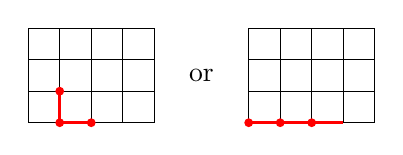
\begin{tikzpicture}[scale=0.4]
  \foreach \s in {0,7} {
  \begin{scope}[xshift=\s cm]
    \foreach \x in {0,...,4} \draw (\x,0) -- (\x,3);
    \foreach \y in {0,...,3} \draw (0,\y) -- (4,\y);
  \end{scope}}
  \draw[red,very thick] (1,1) -- (1,0) -- (2,0);
  \foreach \p in {(1,1),(1,0),(2,0)} \fill[red] \p circle (0.14);
  \draw[red,very thick] (7,0) -- (10,0);
  \foreach \p in {(7,0),(8,0),(9,0)} \fill[red] \p circle (0.14);
  \node at (5.5,1.5) {or};
\end{tikzpicture}
\diagramcaption{Three-spin interactions on a square or along a lattice axis.}
\end{diagram}

Other effects that can change the critical behavior include lattice defects and
impurities in the material (and these are important effects experimentally).

\subsubsection*{Classical and quantum spins}

A note on the basic physics: although we write the interaction term of a magnetic system
as $\Ham = -J\sum_{\langle ij\rangle}\sigma_i\sigma_j$ or
$-J\sum_{\langle ij\rangle}\mathbf{S}_i\cdot\mathbf{S}_j$, the underlying physics is the
Pauli exclusion principle, which for a FM prefers spin alignment to keep the spins apart
and hence reduce the Coulomb repulsion energy. The magnitude of the $J$ is thus set by
the electrostatic Coulomb interaction, not by the dipole--dipole interaction of
individual electrons, which is much smaller.

Another comment concerns the use of classical quantities in stat.\ mech.\ models. The
true interaction that is responsible for magnetic behavior involves quantum mechanics
(QM), and hence the spins are operators, and the Hamiltonian $\Ham$ is a quantum
mechanical operator, not a scalar. However, the behavior of the system can often be well
described by using classical spins. So for a magnet with a largely uniaxial effective
spin--spin interaction, we have
$(S_z)_i(S_z)_j = ((1/2)\sigma_z)_i((1/2)\sigma_z)_j$, and since
$\sigma_z = \left(\begin{smallmatrix}1&0\\0&-1\end{smallmatrix}\right)$, we can replace
these operators by just $\sigma_i\sigma_j$ when the $\sigma_i$ are classical variables
$=\pm 1$ (absorbing the prefactor of $(1/2)^2$ in $J$). Note that the QM commutation
relation
\begin{equation}
  [S_\alpha,S_\beta] = \ii\epsilon_{\alpha\beta\gamma}S_\gamma,\qquad
  \alpha,\beta,\gamma = x,y,z,
\end{equation}
means that $(S_z)_i$ and $(S_z)_j$ commute. This is also true when one has an external
magnetic field in the $\hat{\mathbf{z}}$ direction. Moreover, in the two other examples
of systems in the Ising universality class given above, namely the liquid--gas transition
and the structural phase transition of a binary alloy like brass, the variable
$\sigma_i = \pm 1$ (equivalently $(1+\sigma_i)/2 = 1$ or $0$) refers to an
occupation number, not a spin.

Example of a quantum spin system: the ``transverse Ising model'' with
\begin{equation}
  \Ham = -J\sum_{\langle ij\rangle}(\sigma_z)_i(\sigma_z)_j - \mu H_x\sum_i(\sigma_x)_i ,
\end{equation}
where one applies an external magnetic field transverse to the axis of quantization of
the interacting spins. Because of its complexity, one often studies it in one dimension,
as a ``quantum spin chain''. Studies go back to the 1920s and 1930s, e.g.\ by Bethe and
others. For examples, see, e.g.:
\begin{itemize}
  \item B.~McCoy, J.~Perk, R.~Shrock, Nucl.\ Phys.\ \textbf{B220}, 35 (1983);
    \textbf{B220}, 269 (1983);
  \item G.~M\"uller and R.~Shrock, Phys.\ Rev.\ Lett.\ \textbf{51}, 219 (1983);
    Phys.\ Rev.\ B \textbf{29}, 288 (1984);
\end{itemize}
also papers by Profs.\ V.~Korepin, Tzu-Chieh Wei, and Nat Tantivasadakarn.

There has been a resurgence of interest in quantum spin systems via the application to
quantum computing. We recommend the courses in quantum computing taught here (Korepin,
Wei, Tantivasadakarn, \ldots).
